Results for the accuracy of alternative distribution parameters $\pi_1$ and $\mu_1$ are shown in Figure \ref{SIM_model}.  We can see that for very small effect sizes, the prevalence of activation $\pi_1$ is unbiased, while for medium to large effect sizes $\pi_1$ is overestimated.  We show in the supplementary materials that this effect can be explained by the mismatch between the modeled beta-distribution and the observed distribution of $p$-values for active peaks.

Effect size tends to be underestimated, especially for the sparsest activations.  When only few activation areas are present, the number of activated peaks is very small in relation to the number of null peaks and the mixture model can struggle to separate distributions.
With larger activation areas, the underestimation is reduced.

\begin{center}
\begin{figure}[h]
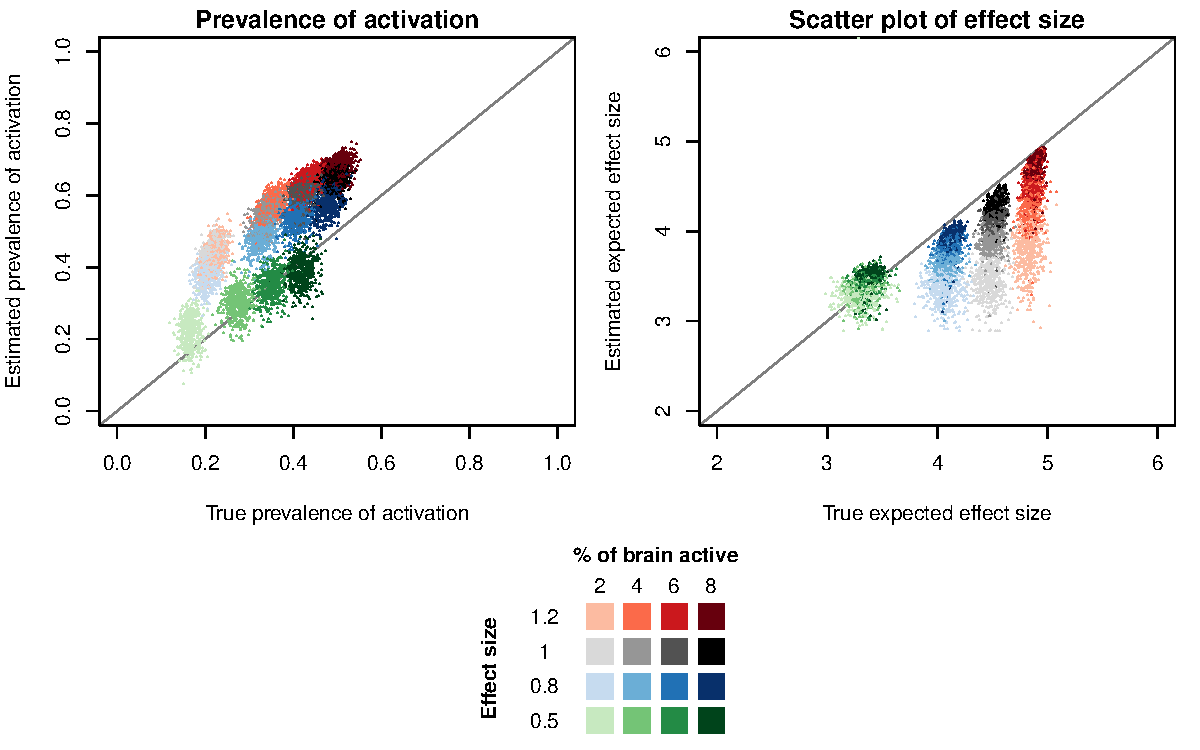
\includegraphics[scale=0.8]{figures/FIG_SIM_modelestimation_15_NOMASK_2_5.pdf}
\caption{Left: Plot of estimated $\hat\pi_1$ against true $\pi_1$ for different sample sizes and different values for $\mu_1$. Each dot represents a different simulation, as such there are 500 dots for each condition.  Right: Plot of estimated expected peak height $\hat{E}(Z_j^u)$ against true expected peak height $\widetilde{E}(Z_j^u)$ for different effect sizes. The estimations are the result for a pilot dataset with $n=15$.  \label{SIM_model}}
\end{figure}
\end{center}

Using these estimates of $\pi_1$, $\mu_1$ and $\sigma_1$ for the case of $n=15$, we then computed power for future studies for peak inference with 5\% error rate control for the different inference procedures tested (see section \ref{threshold}). Figure \ref{SIM_pow} shows the plot of $(1-\hat\beta_z)$ and $(1-\widetilde\beta_z)$ for {\color{Cyan}$n^*=15,...,60$}. In all conditions, but increasingly with small (local) activated brain regions, the power is largely underestimated.  This leads to conservative results.
For larger activated regions, the results are less conservative.  As expected, the power is overestimated for FDR control.
%The procedure is often unable to estimate power for FDR thresholding for smaller effect sizes.  This is because - due to the adaptive character of the procedure - in the pilot study often no significant effects are found.  Therefore, there is no cutoff, and as such power cannot be estimated in larger sample sizes. The non-adaptive multiple testing procedures show a modest bias only.

\begin{center}
\begin{figure}[h]
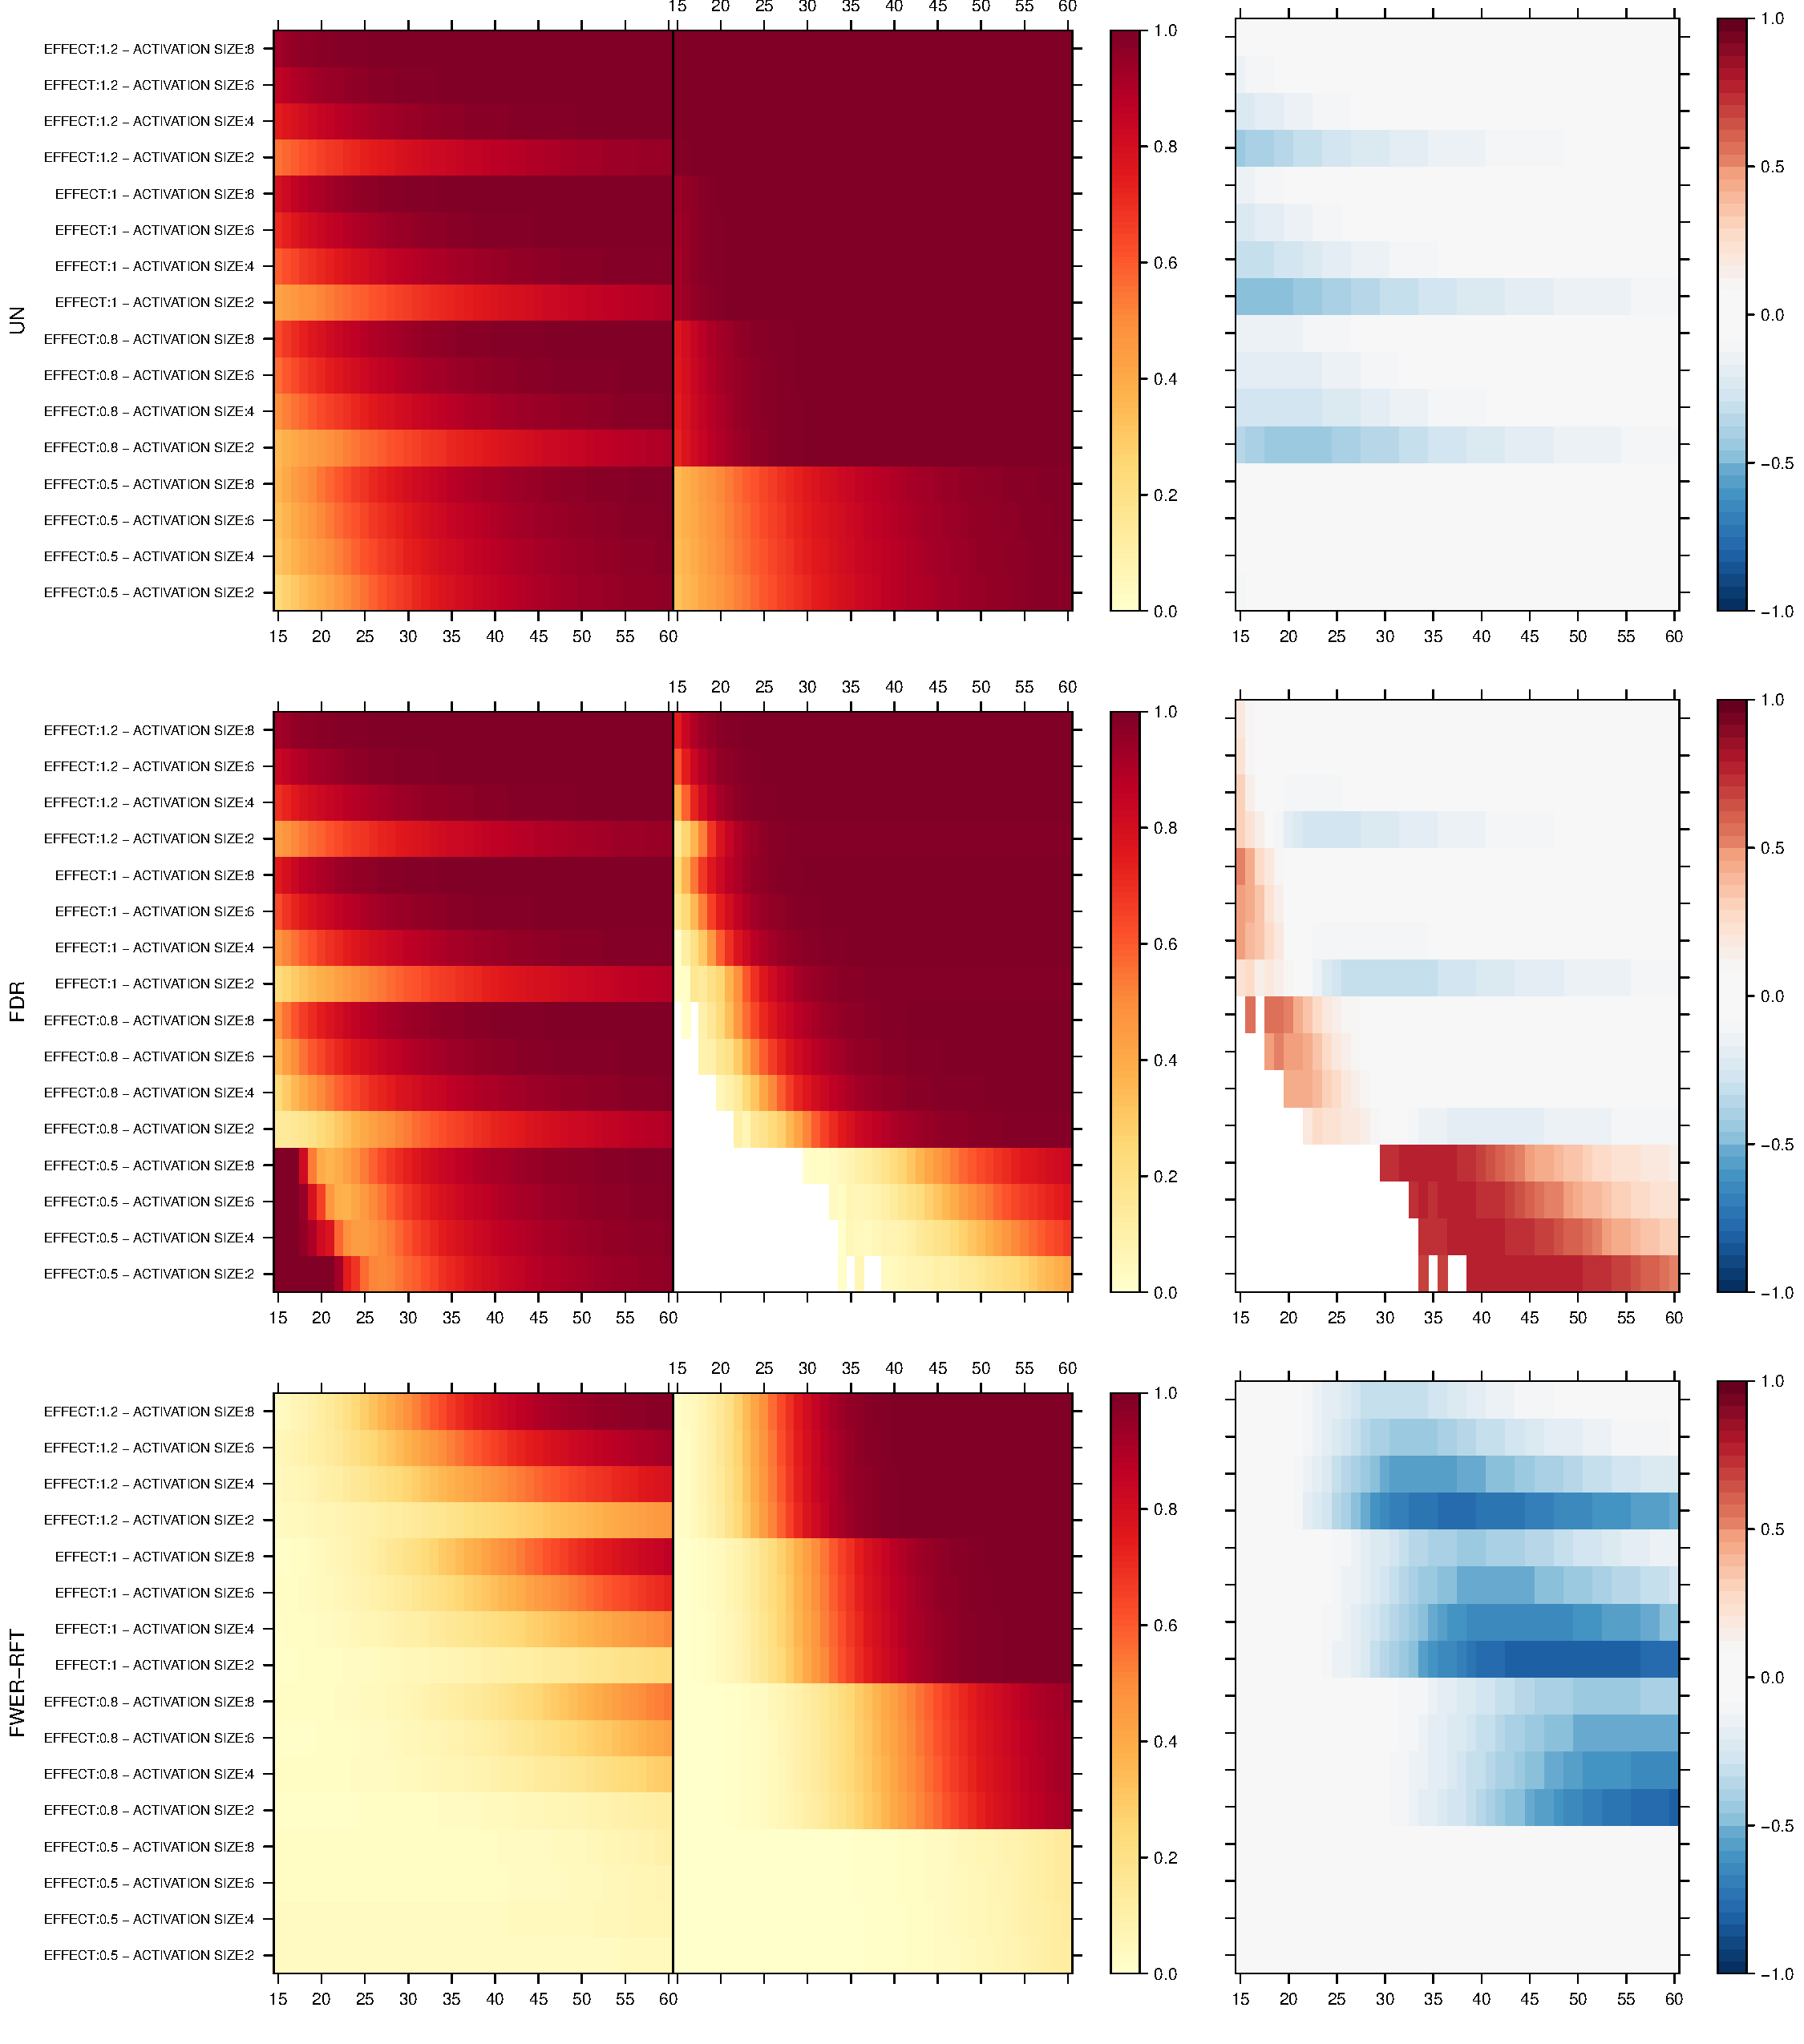
\includegraphics[scale=0.4]{figures/FIG_SIM_power_15_NOMASK_2_5.pdf}
\caption{Plots of the peakwise average power with error rate control at 5\% for different effect sizes and different amounts of activation.  The left column shows the estimated power curves, the middle column shows the true power and the right column shows the bias.  Bias is defined as the estimated power minus the true power.  The peakwise average power is estimated from a pilot study with 15 subjects. \label{SIM_pow}}
\end{figure}
\end{center}

Due to the increasing conservativism with more local effect sizes, we repeated the power calculation method using a mask that covers 28 percent of the full map.  The results, shown in Figure \ref{SIM_pow_mask} indeed indicate that the estimation of the model and power is better using a mask.

\begin{center}
\begin{figure}[h]
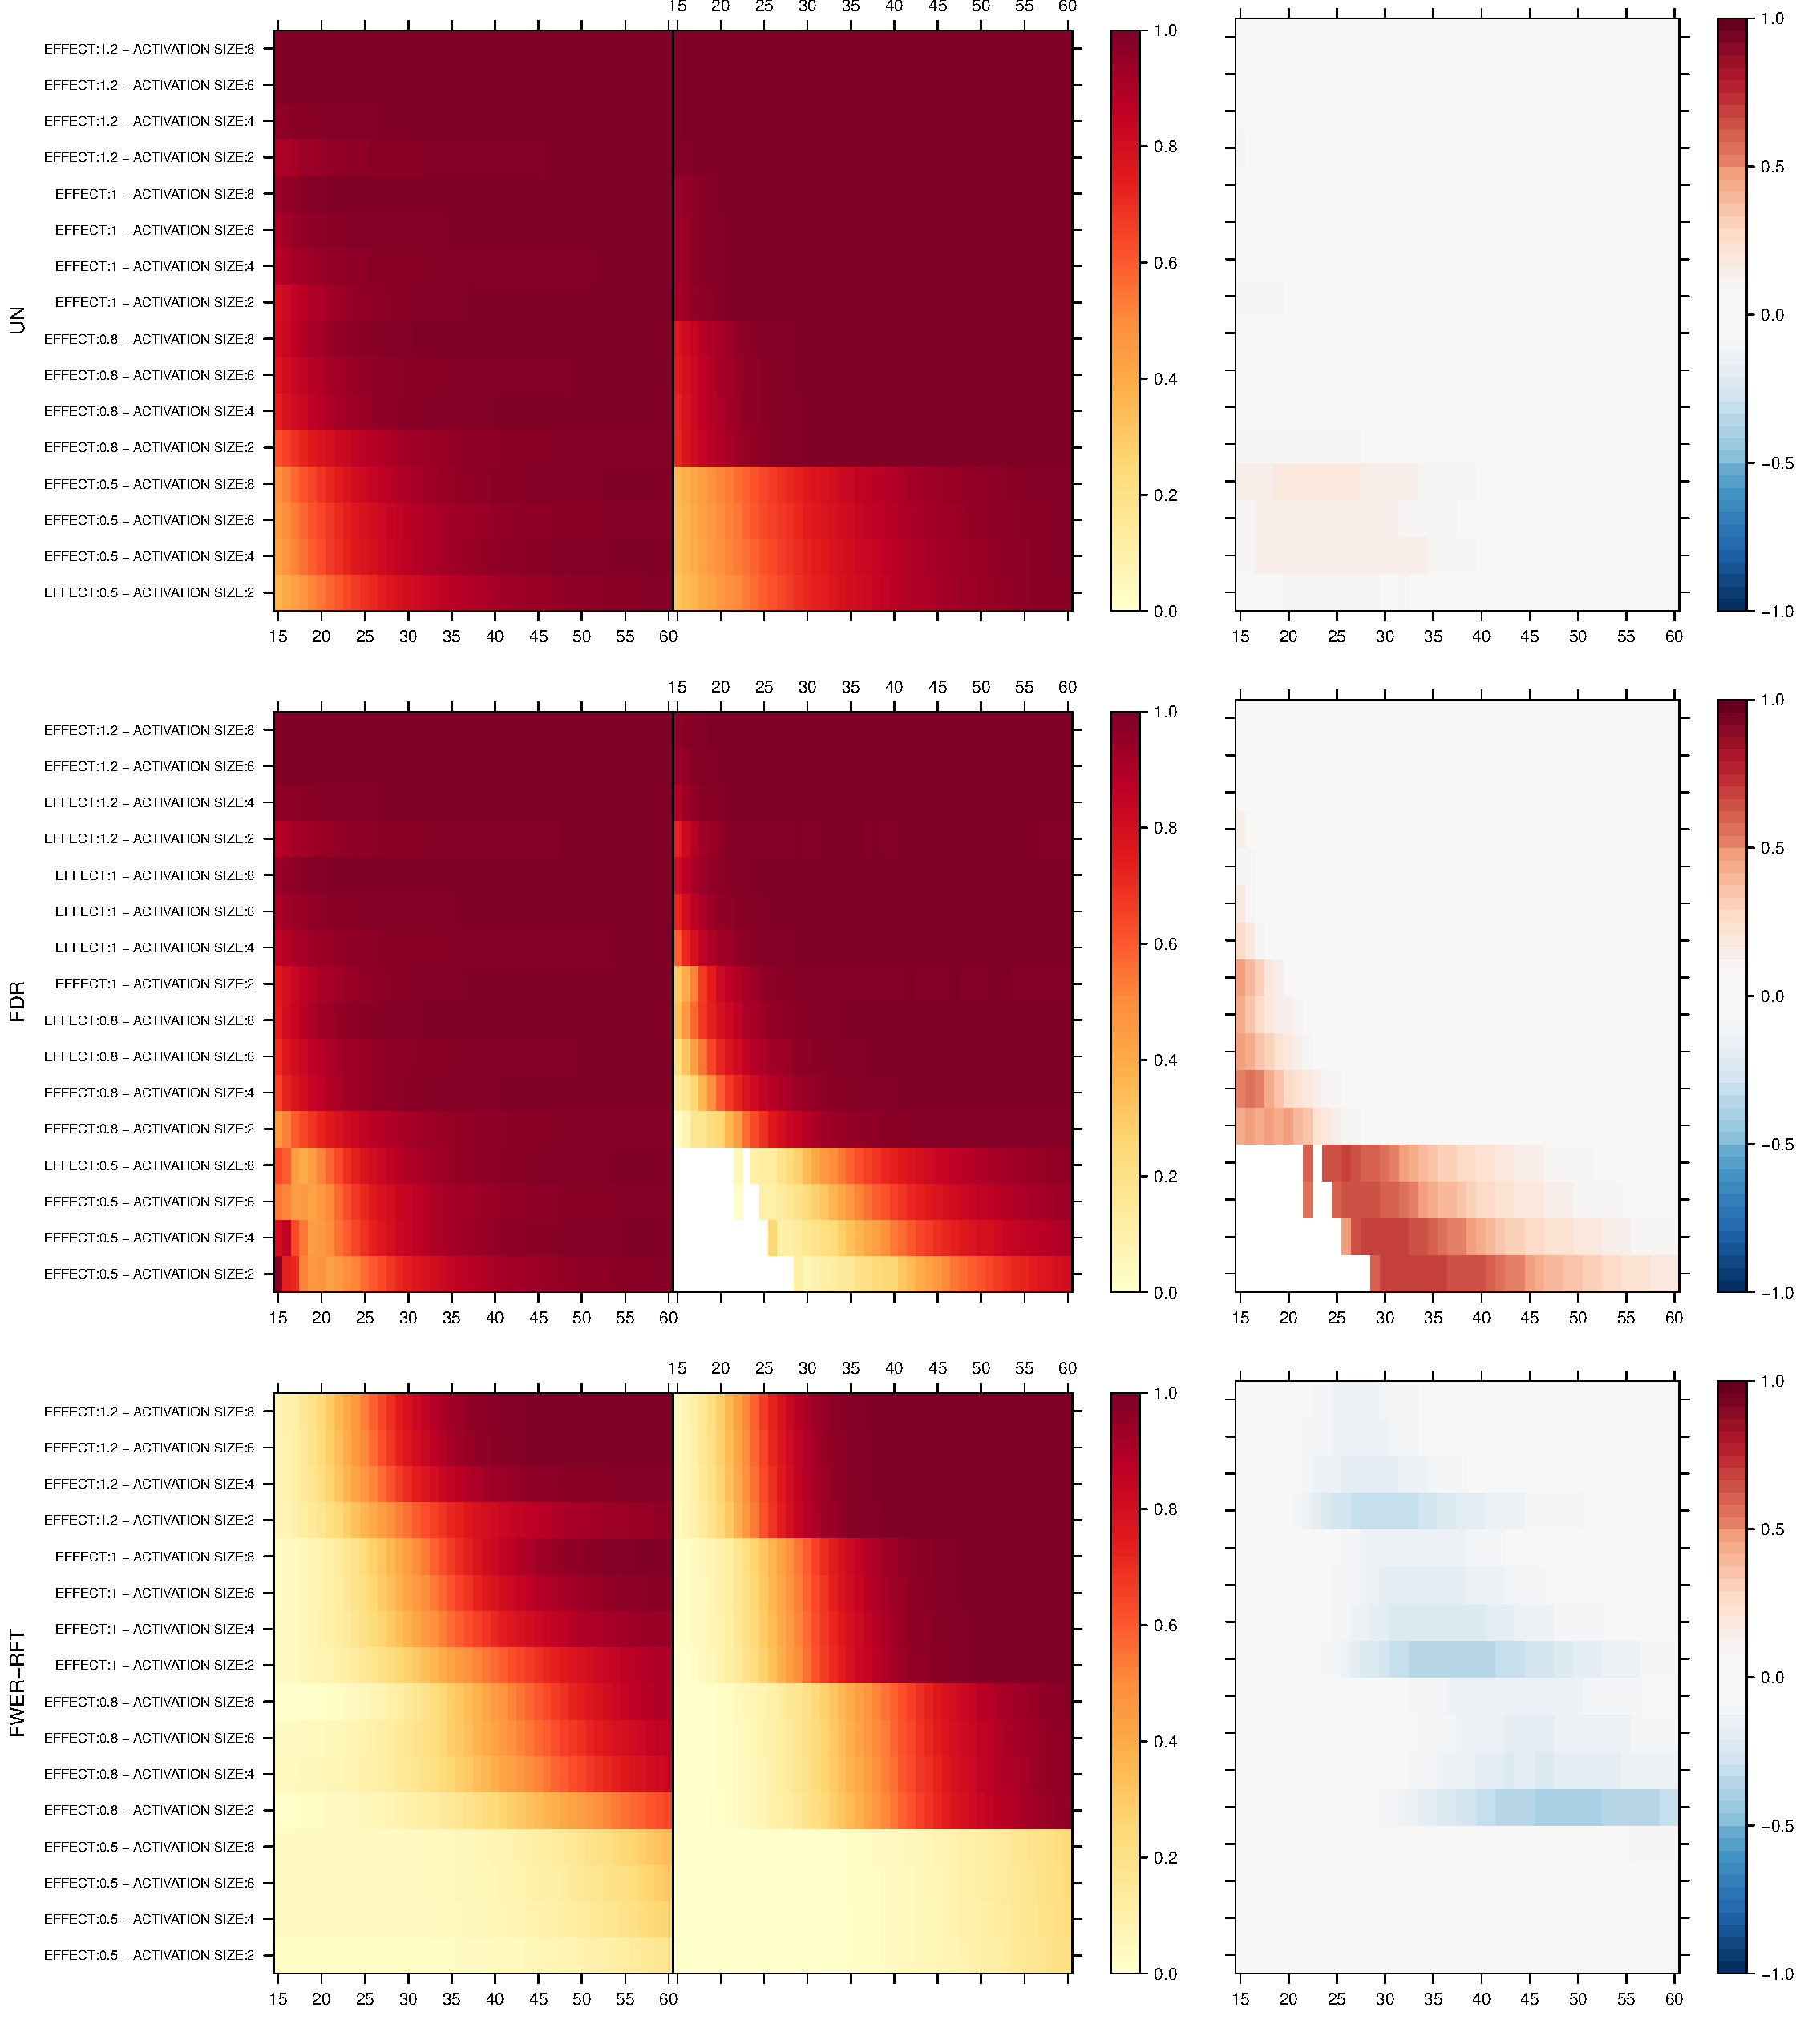
\includegraphics[scale=0.4]{figures/FIG_SIM_power_15_MASK_2_5.pdf}
\caption{Plots of the peakwise average power with error rate control at 5\% for different effect sizes and different amounts of activation, using a mask covering about 1/4th (28\%) of the original map.  The left column shows the estimated power curves, the middle column shows the true power and the right column shows the bias.  Bias is defined as the estimated power minus the true power.  The peakwise average power is estimated from a pilot study with 15 subjects. \label{SIM_pow_mask}}
\end{figure}
\end{center}

The goal of the presented method is to perform sample size calculations.  Figure \ref{SIM_ss} shows the performance of these sample size calculations when 80\% power is desired.  While the variance is high for conditions with small effect sizes, the average bias of most conditions and multiple comparison procedures is within a range of 5 subjects.  We immediately show results using the masks described in the previous paragraph.

\begin{center}
\begin{figure}[h]
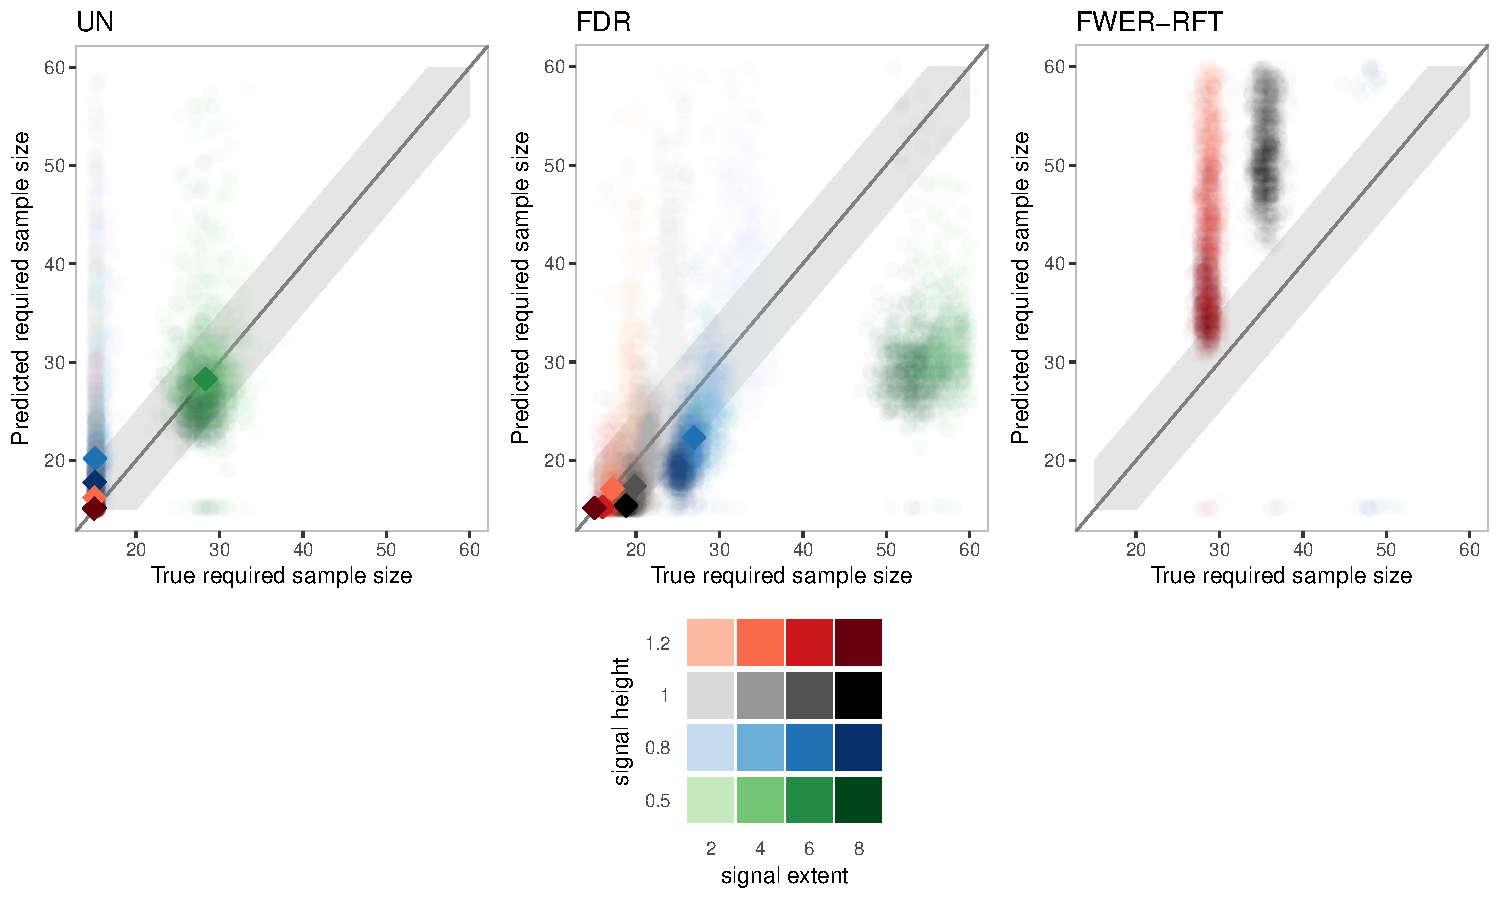
\includegraphics[scale=0.5]{figures/FIG_SIM_sscalc_15_NOMASK_2_5.pdf}
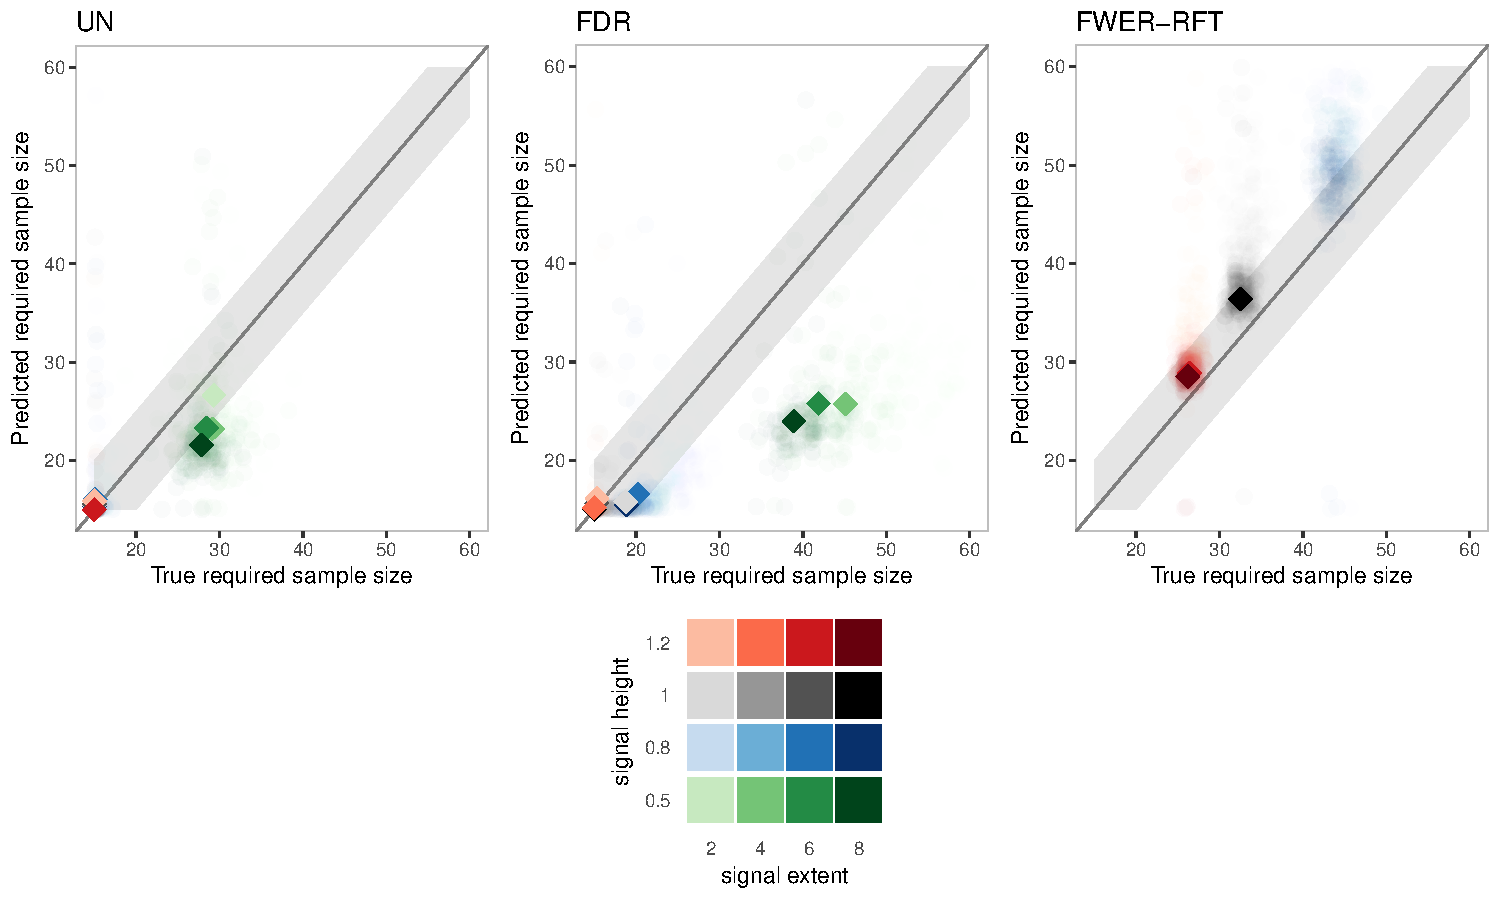
\includegraphics[scale=0.5]{figures/FIG_SIM_sscalc_15_MASK_2_5.pdf}
\caption{Plots of the predicted and true required sample size when 80\% power is desired. The upper plot shows the results without applying a mask, the lower plot shows the results with mask.  The different plots refer to the different multiple testing procedures.  Points inside the grey area identify points with a maximum bias of 5 subjects.  Each semi-transparent dot represents a different simulation, as such there are 500 dots for each condition.  The fully colored dots present the average per condition.  The estimated sample size results from a pilot study with 15 subjects. \label{SIM_ss}}
\end{figure}
\end{center}
